\section{PicoBlaze Realisierung}
% For special Enumeration in this chapter--------------
\newcommand*\circled[1]{
    \tikz[baseline=(char.base)]{
        \node[shape=circle,draw,inner sep=0pt] (char) {#1\strut}
    }\kern-3pt
}

\let\oldlabelenumi=\labelenumi
\let\oldlabelenumii=\labelenumii
%------------------------------------------------------
\subsection{Instruction- Zyklus und -Abarbeitung}
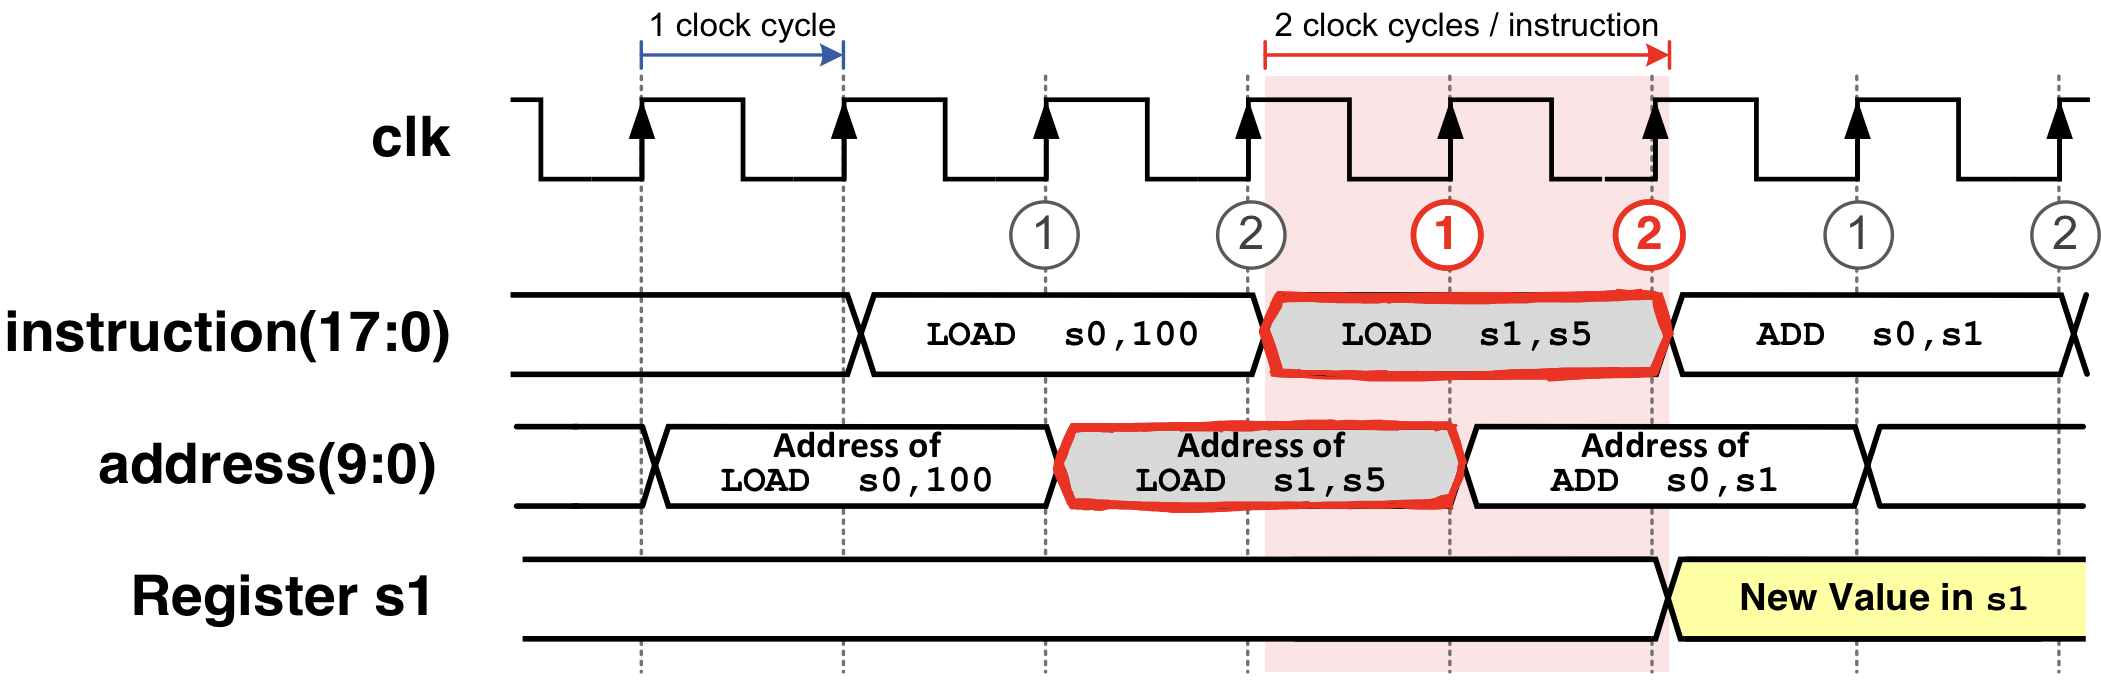
\includegraphics[width=12cm]{pics/7-Instruktion-zyklus}
\begin{enumerate}
	\setcounter{enumi}{1}
	\renewcommand{\labelenumi}{\circled{\oldlabelenumi}}
		\item Die vorangegangene Instruktion LOAD s0, 100 ist ausgef"uhrt und abgeschlossen, die Adresse der Instruktion \color{red} LOAD s1, s5 \color{black} wird auf \textit{\textbf{address(9:0)}} angelegt.
	\renewcommand{\labelenumi}{\oldlabelenumi}
	\color{red}
	\setcounter{enumi}{0}
	\renewcommand{\labelenumi}{\circled{\oldlabelenumi}}
		\item \color{black} Die Instruktion \color{red} LOAD s1, s5 \color{black} wird auf \textit{\textbf{instruction(17:0)}} vom Block\_RAM zum CORE "ubertragen.
	\renewcommand{\labelenumi}{\oldlabelenumi}
	\color{red}
	\renewcommand{\labelenumi}{\circled{\oldlabelenumi}}
		\item \color{black} Die Instruktion \color{red} LOAD s1, s5 \color{black} wird ausgef"uhrt und abgeschlossen, damit wird im Register \textbf{s1} der neue Wert verf"ugbar. Die Adresse der n"achsten Instruktion wird auf auf \textit{\textbf{address(9:0)}} angelegt.
	\renewcommand{\labelenumi}{\oldlabelenumi}
	\setcounter{enumi}{0}
	\renewcommand{\labelenumi}{\circled{\oldlabelenumi}}
		\item usw.
	\renewcommand{\labelenumi}{\oldlabelenumi}
\end{enumerate}

\subsection{Input Ports}
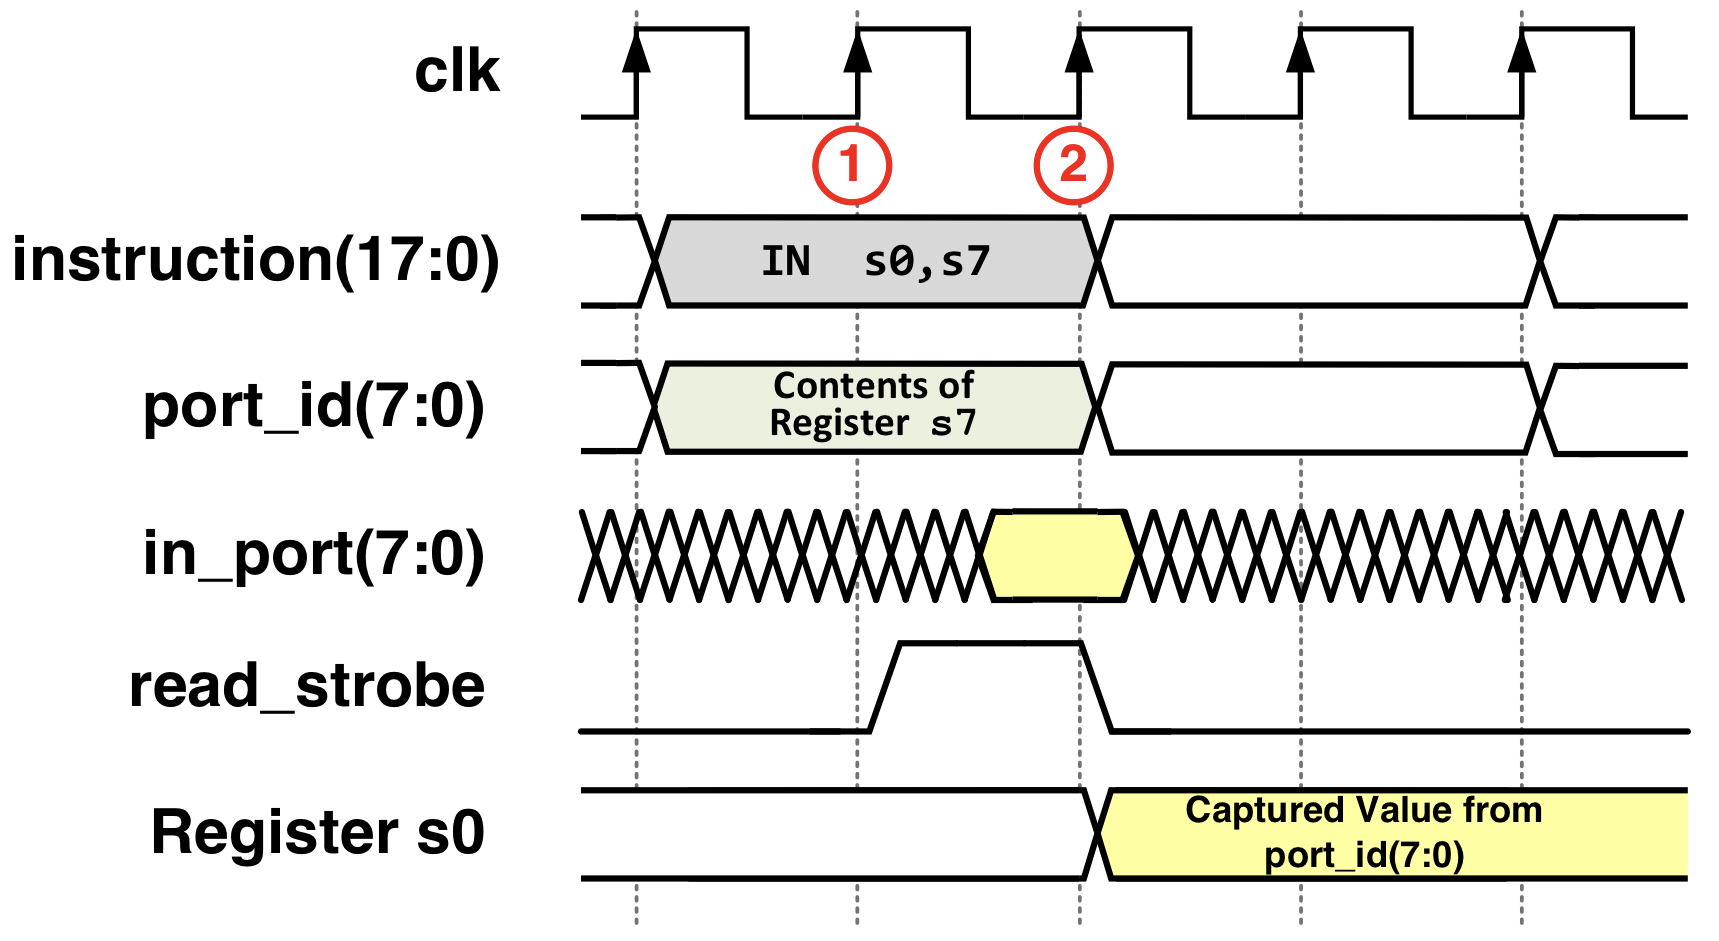
\includegraphics[width=8cm]{pics/7-Input-Ports_Timing}
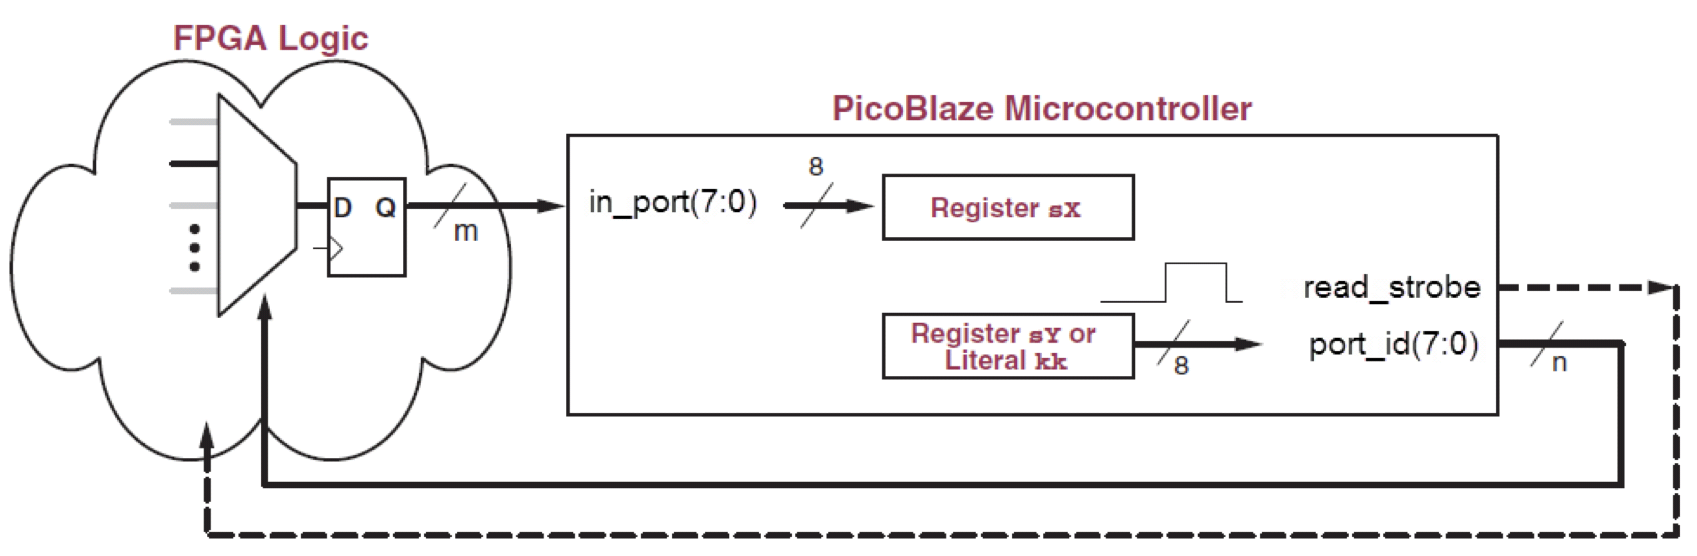
\includegraphics[width=11cm]{pics/7-Input-Ports_Logik}
\begin{enumerate}
	\color{red}
	\renewcommand{\labelenumi}{\circled{\oldlabelenumi}}
		\item \color{black} Die in der \color{red} \textbf{IN} \color{black} Instruktion spezifizierte Port Address wird auf \textit{\textbf{port\_id(7:0)}} ausgegeben. "Uber \textit{\textbf{read\_strobe}} wird der FPGA-Logic die g"ultige Port-Address signalisiert. Damit kann der Multiplexer die Daten auf \textit{\textbf{in\_port(7:0)}} bereitlegen.
	\renewcommand{\labelenumi}{\oldlabelenumi}
	\color{red}
	\renewcommand{\labelenumi}{\circled{\oldlabelenumi}}
		\item \color{black} Die am Input Data Port bereit liegenden Daten werden "uber \textit{\textbf{in\_port(7:0)}} eingelesen und im spezifizierten Register abgelegt. \textit{\textbf{read\_strobe}} wird deaktiviert.
	\renewcommand{\labelenumi}{\oldlabelenumi}
\end{enumerate}
\newpage

\subsection{Output Ports}
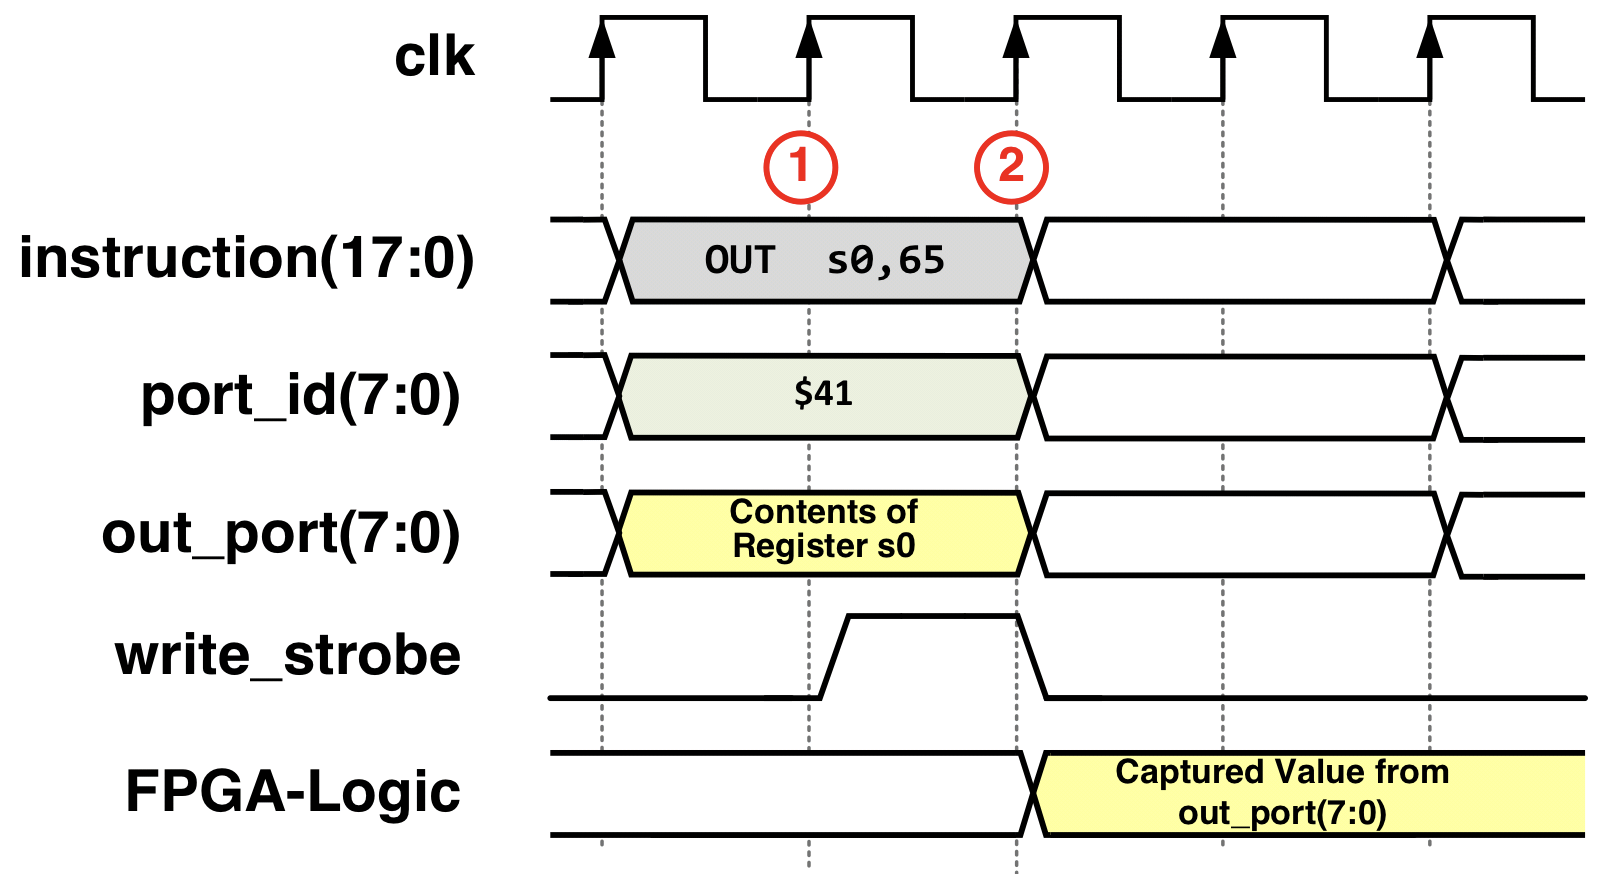
\includegraphics[width=8cm]{pics/7-Output-Ports_Timing}
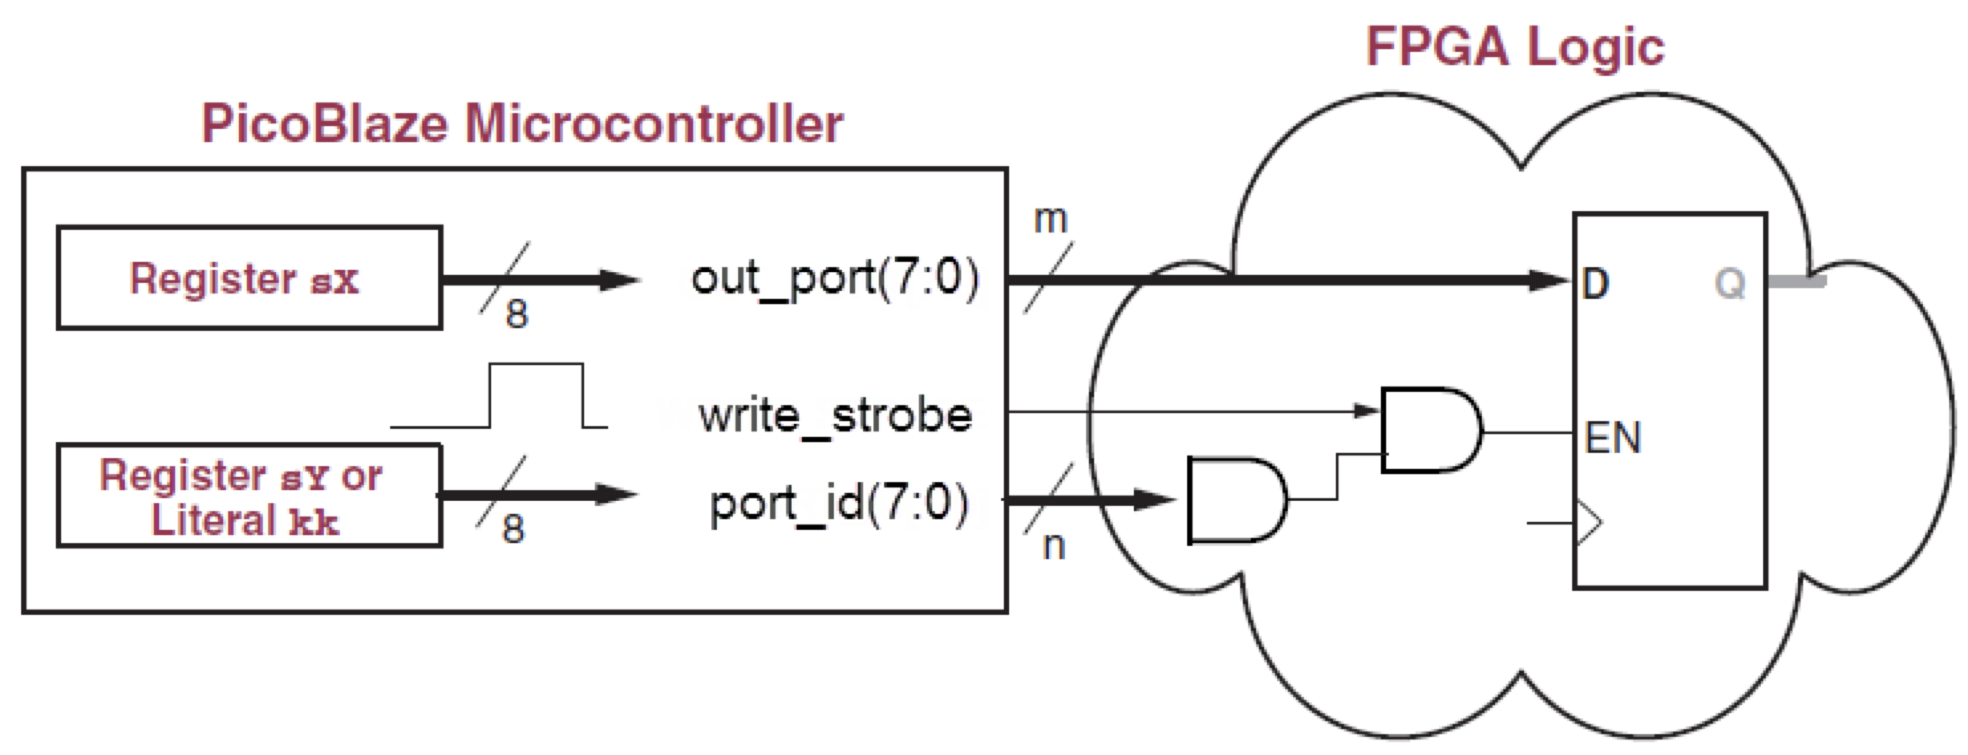
\includegraphics[width=10cm]{pics/7-Output-Ports_Logik}
\begin{enumerate}
	\color{red}
	\renewcommand{\labelenumi}{\circled{\oldlabelenumi}}
		\item \color{black} Die in der \color{red} \textbf{OUT} \color{black} Instruktion spezifizierte Port Address wird auf \textit{\textbf{port\_id(7:0)}} ausgegeben. "Uber \textit{\textbf{write\_strobe}} wird der FPGA-Logic die g"ultige Port-Address signalisiert. Die FPGA-Logik kann sich so bereits vorbereiten, die Daten bei der n"achsten steigenden Clock-Flanke zu "ubernehmen.
	\renewcommand{\labelenumi}{\oldlabelenumi}
	\color{red}
	\renewcommand{\labelenumi}{\circled{\oldlabelenumi}}
		\item \color{black} Die am Output Data Port \textit{\textbf{out\_port(7:0)}} bereit stehenden Daten werden von der FPGA-Logic entgegengenommen.\textit{\textbf{write\_strobe}} wird deaktiviert.
	\renewcommand{\labelenumi}{\oldlabelenumi}
\end{enumerate}

\subsection{Interrupts}
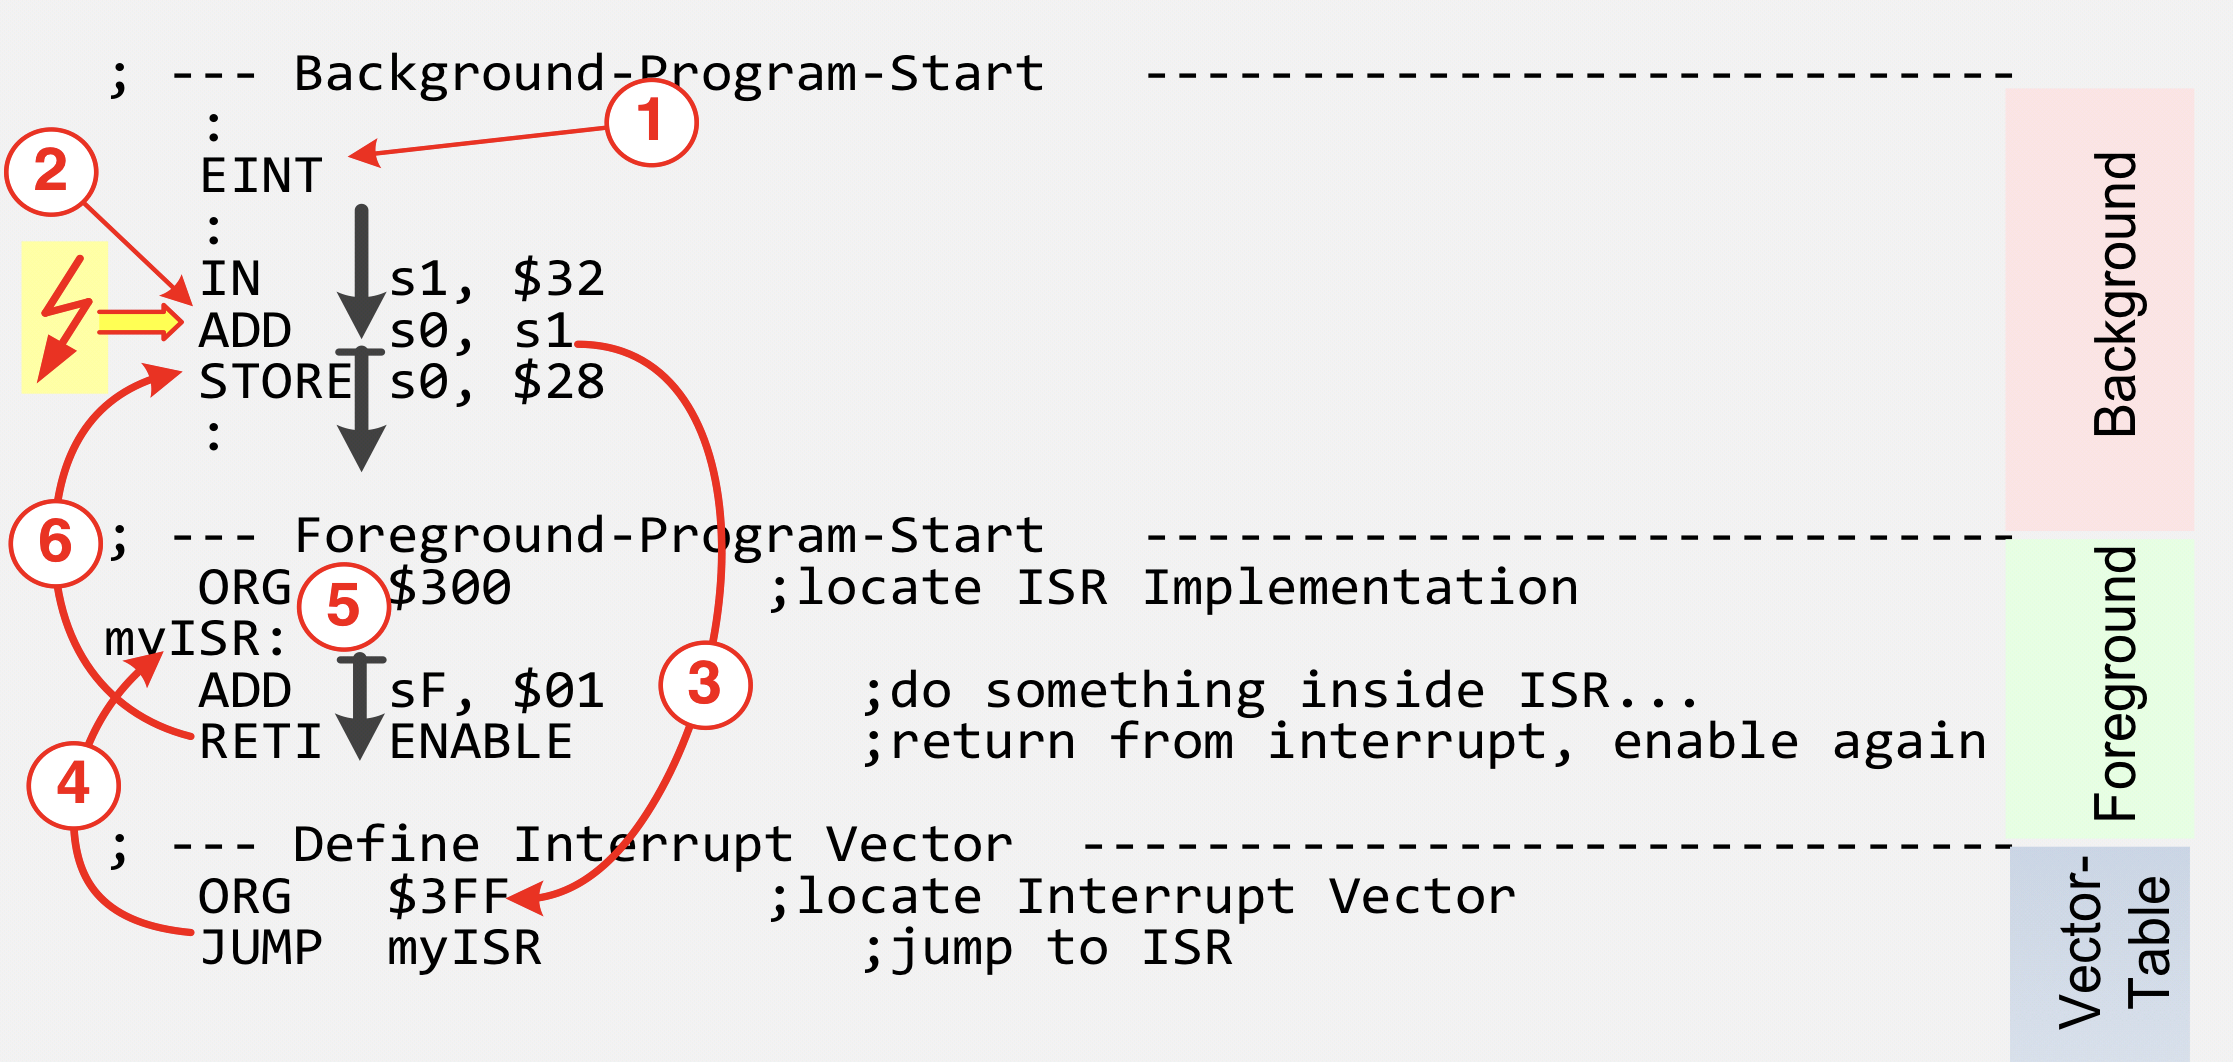
\includegraphics[width=12cm]{pics/7-Interrupts_Code}

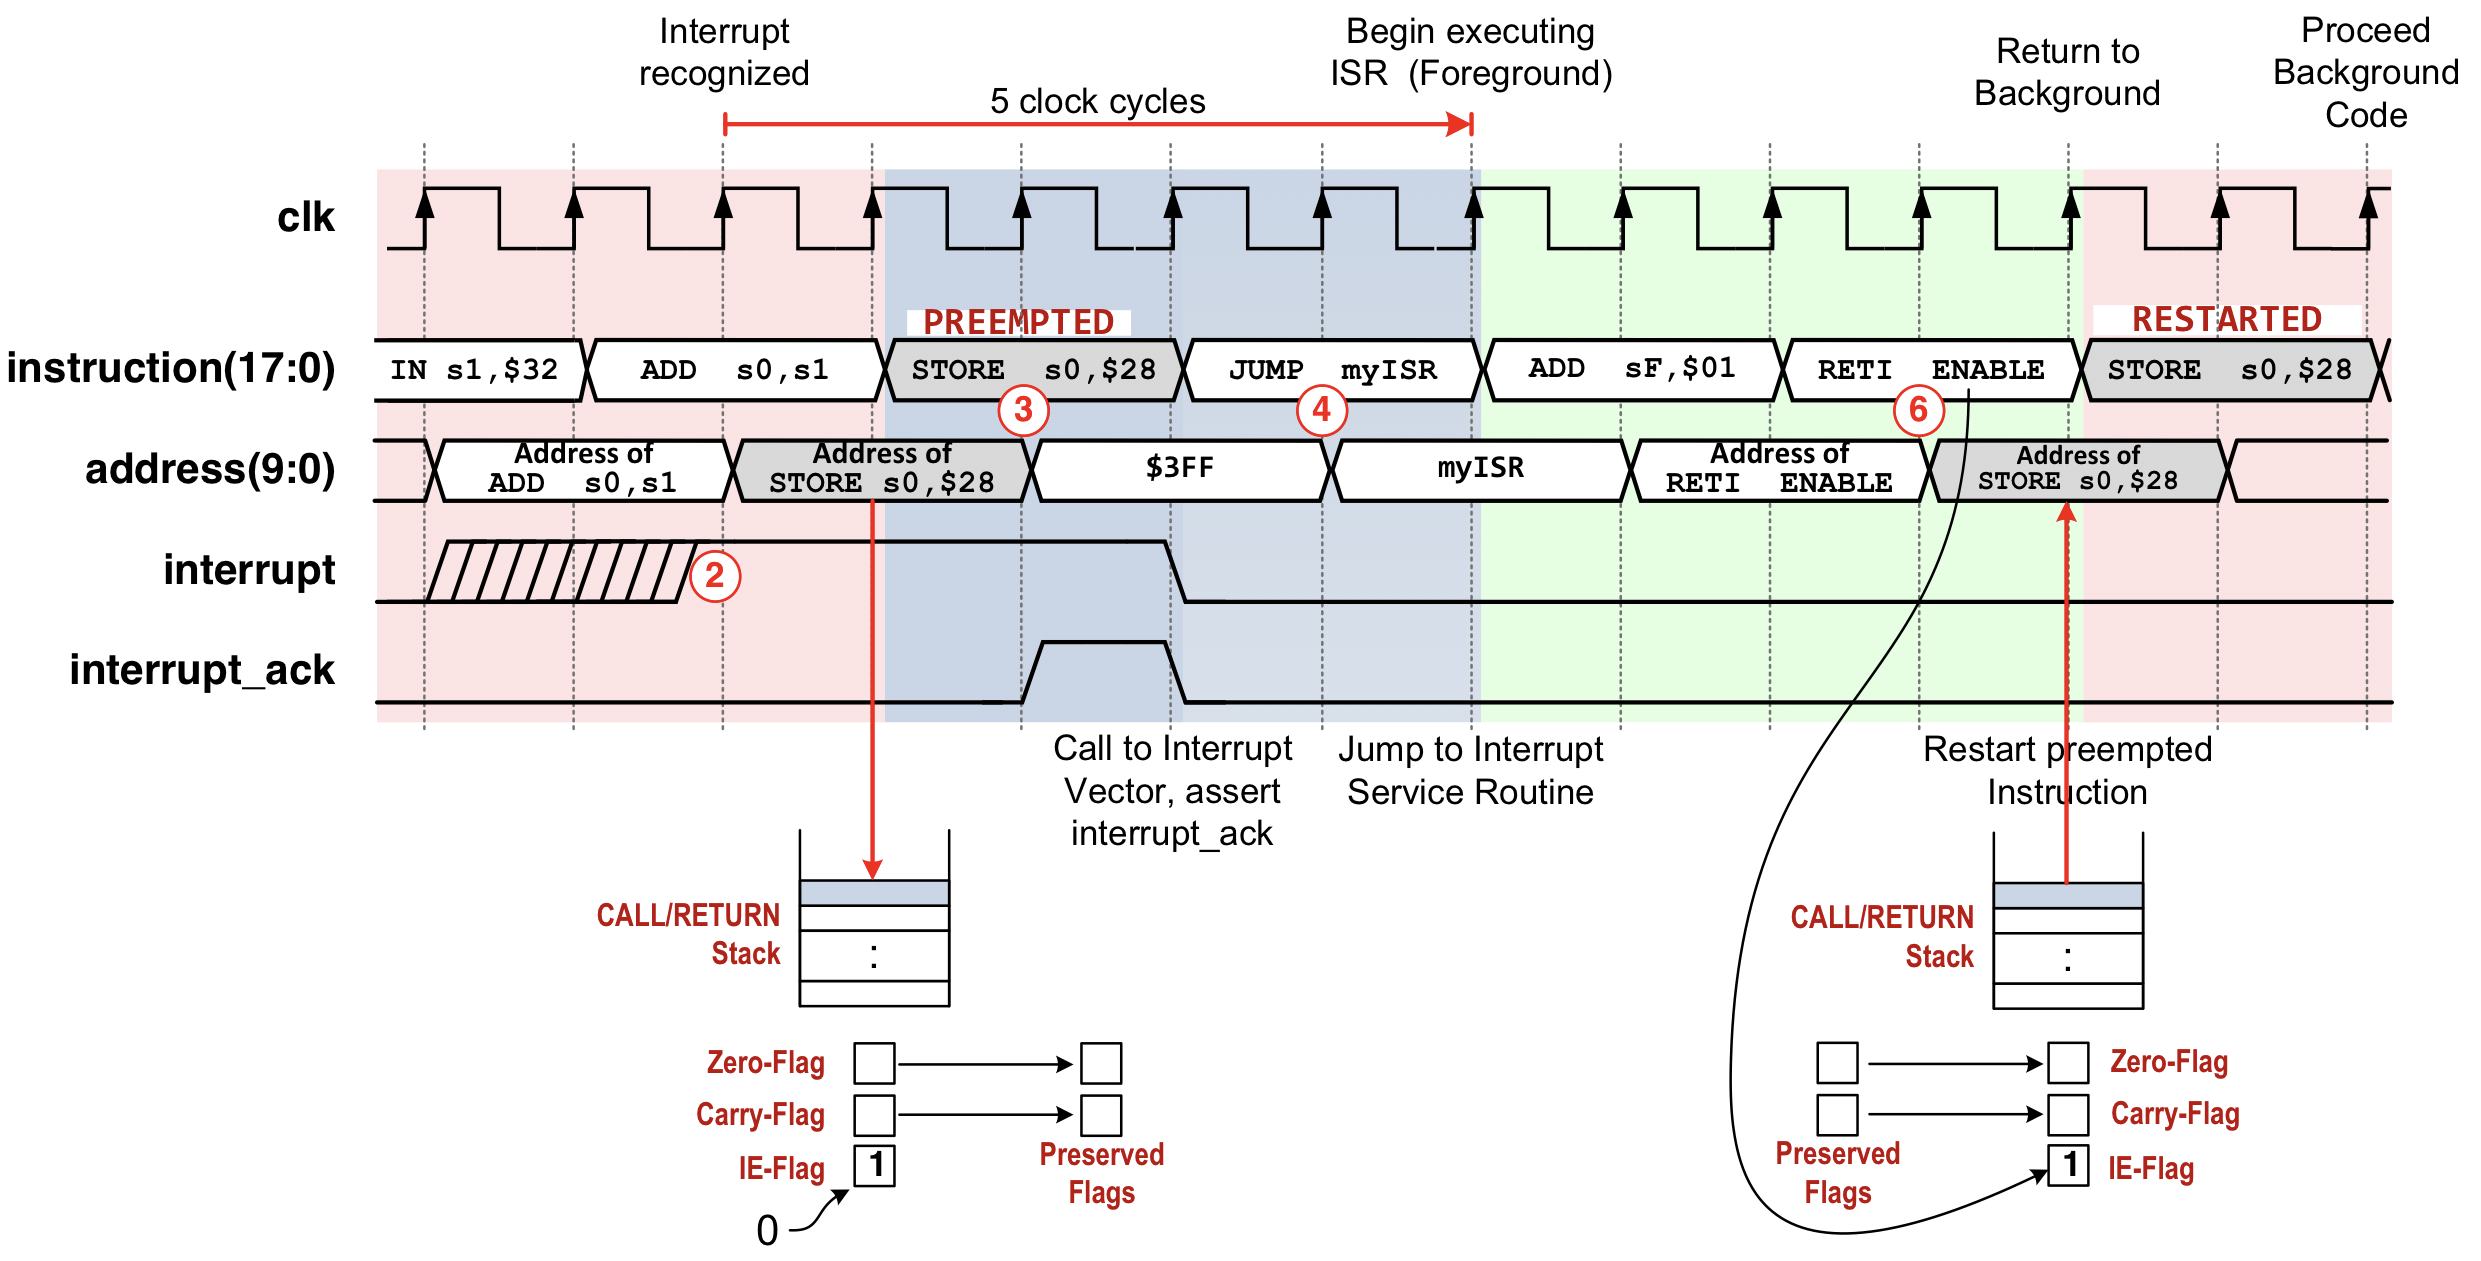
\includegraphics[width=18cm]{pics/7-Interrupts_Timing}

Der Interrupt wird bei \color{red}\circled{2}\color{black} \ \ in einem FlipFlop gespeichert. Der Ausgang des FFs ist mit dem Interrupt-Eingang des PicoBlaze verbunden. Bei \color{red}\circled{3}\color{black} \ \ wird das FF durch den \textbf{interrupt\_ack} des PicoBlaze zur"uckgesetzt.